\documentclass[border=.1cm]{standalone}

\usepackage{tikz}
\usepackage{times}
\usepackage{pgfplots}
\usepgflibrary{arrows}

\usepackage{siunitx}
\sisetup{
    detect-all = true,
    input-decimal-markers = {.},
    input-ignore = {,},
    inter-unit-product = \ensuremath{{}\cdot{}},
    multi-part-units = repeat,
    number-unit-product = \text{~},
    per-mode = fraction,
    separate-uncertainty = true,
}

\begin{document}

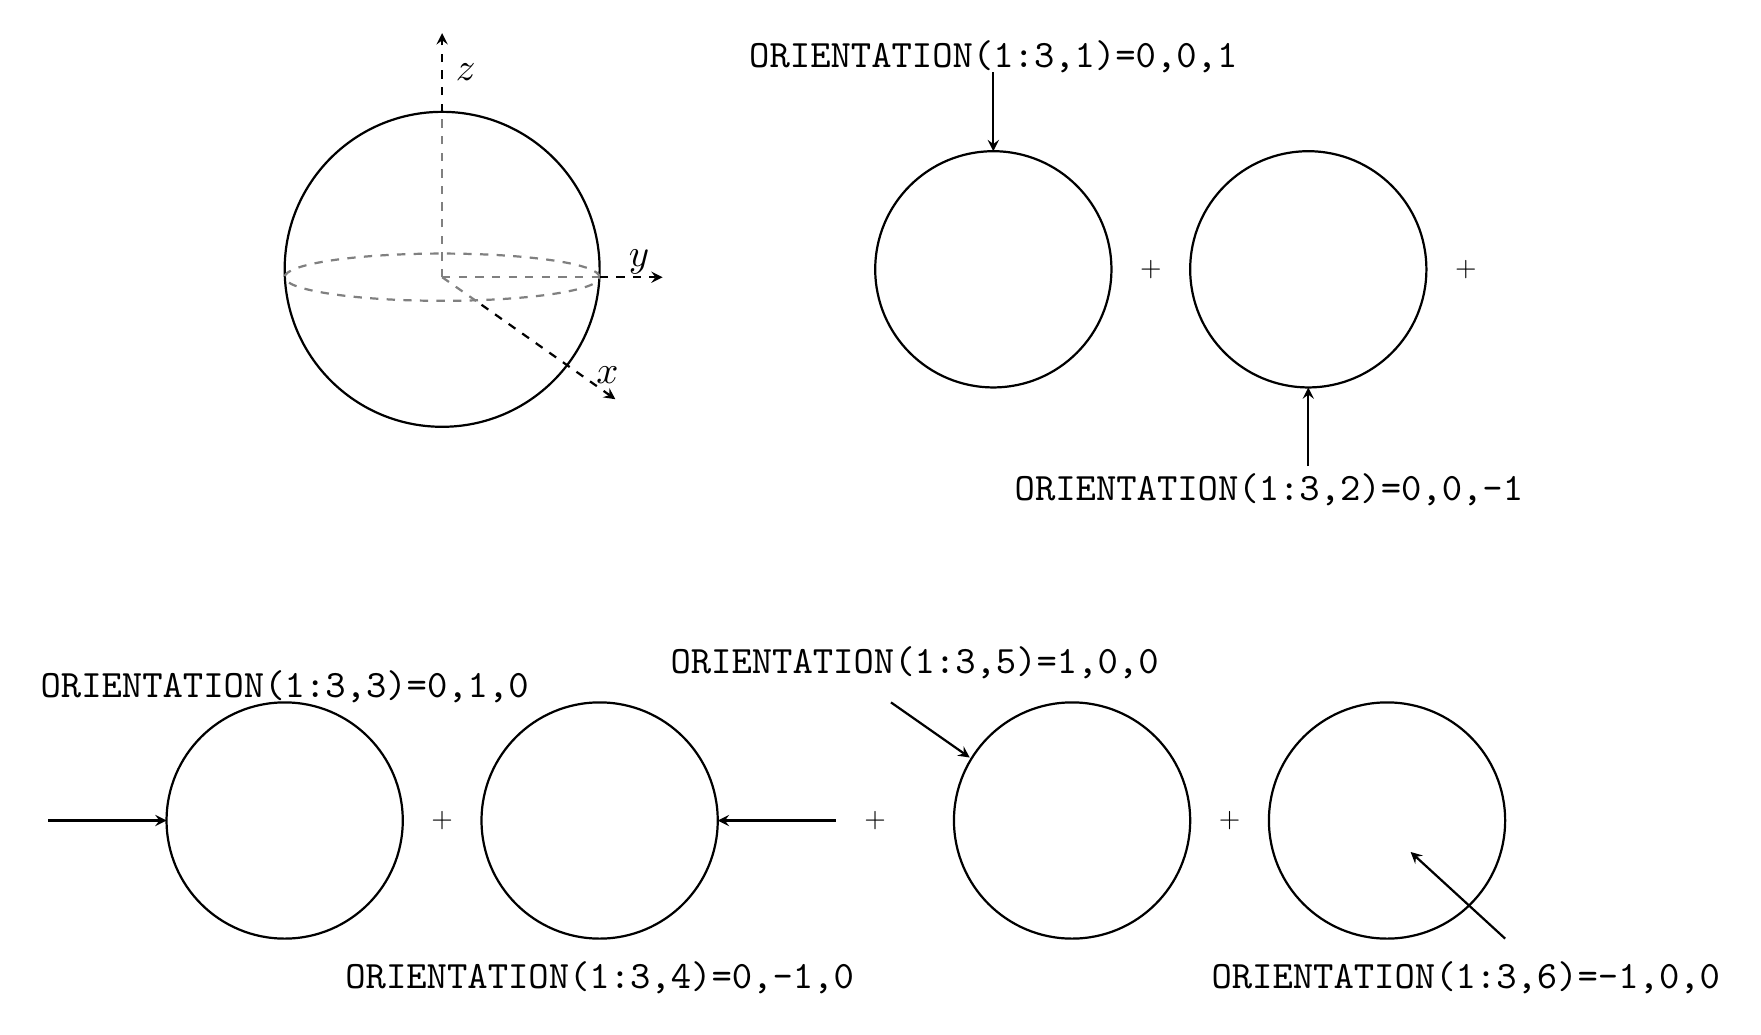
\begin{tikzpicture}

\draw [thick](0,0) circle (1.5cm);
\node at (0, 1.7)[thick,scale = 1.4]{\tt ORIENTATION(1:3,3)=0,1,0};
\draw[-stealth,thick](-3,0) -- (-1.5,0);

\node at (2,0){+};

\draw [thick](4,0) circle (1.5cm);
\node at (4, -2)[thick,scale = 1.4]{\tt ORIENTATION(1:3,4)=0,-1,0};
\draw[-stealth,thick](7,0) -- (5.5,0);

\node at (7.5,0){+};

\draw [thick](10,0) circle (1.5cm);
\node at (8,2)[thick,scale = 1.4]{\tt ORIENTATION(1:3,5)=1,0,0};
\draw[-stealth,thick](7.7,1.5) -- (8.7,.8);

\node at (12,0){+};

\draw [thick](14,0) circle (1.5cm);
\node at (15,-2)[thick,scale = 1.4]{\tt ORIENTATION(1:3,6)=-1,0,0};
\draw[-stealth,thick](15.5,-1.5) -- (14.3,-.4);

\draw [thick](9,7) circle (1.5cm);
\node at (9,9.7)[thick,scale = 1.4]{\tt ORIENTATION(1:3,1)=0,0,1};
\draw[-stealth,thick](9,9.5) -- (9,8.5);

\node at (11,7){+};

\draw [thick](13,7) circle (1.5cm);
\node at (12.5,4.2)[thick,scale = 1.4]{\tt ORIENTATION(1:3,2)=0,0,-1};
\draw[-stealth,thick](13,4.5) -- (13,5.5);

\node at (15,7){+};

\draw [thick](2,7) circle (2cm);
\draw[gray,dashed,thick](2,6.9) ellipse(2cm and .3cm);
\draw[gray,dashed,thick](2,6.9) -- (4,6.9);
\draw[-stealth,dashed,thick](4,6.9) -- (4.8,6.9);
\node at (4.5,7.1)[thick,scale = 1.4]{$y$};
\draw[gray,dashed,thick](2,6.9) -- (2.5, 6.55);
\draw[-stealth,dashed,thick](2.5,6.55) -- (4.2, 5.35);
\node at (4.1,5.65)[thick,scale = 1.4]{$x$};
\draw[gray, dashed, thick](2,6.9) -- (2,9.0);
\draw[-stealth,dashed, thick](2,9.0) -- (2,10);
\node at (2.3,9.5)[thick,scale = 1.4]{$z$};

\end{tikzpicture}

\end{document}
